%% ============================================================================
%% Paper 3: Quantum-Inspired Molecular Representations
%% Target: Journal of Cheminformatics
%% Target: Journal of Cheminformatics
%% Updated: July 2026 — benchmark results finalised
%% ============================================================================

\documentclass[11pt,a4paper]{article}

% Page layout
\usepackage[a4paper,margin=2.5cm]{geometry}

% Fonts and encoding
\usepackage[T1]{fontenc}
\usepackage[utf8]{inputenc}
\usepackage{lmodern}

% Mathematics
\usepackage{amsmath, amsfonts, amssymb, mathtools}

% Figures and tables
\usepackage{graphicx}
\usepackage{subfig}
\usepackage{booktabs, tabularx, array, multirow, longtable}
\usepackage[table]{xcolor}
\usepackage{algorithm, algorithmic}

% Units and SI
\usepackage[
  detect-all           = true,
  group-minimum-digits = 4,
  per-mode             = symbol,
  range-phrase         = {--},
  range-units          = single,
]{siunitx}
\DeclareSIUnit\angstrom{\text{\AA}}
\DeclareSIUnit\molar{M}
\DeclareSIUnit\kcalmol{kcal\,mol^{-1}}
\DeclareSIUnit\percent{\%}

% Hyperlinks
\usepackage[authoryear,round]{natbib}
\usepackage[hypertexnames=false,colorlinks=true,linkcolor=blue,citecolor=blue,urlcolor=blue]{hyperref}

% Cross-referencing - load after hyperref
\usepackage{cleveref}
\usepackage{xr}
%% Cross-reference to Paper 2 (companion MD validation study):
%% Commented out for standalone Journal of Cheminformatics submission.
%% \externaldocument[P2-]{../../Project2_Polypharmacology_MD_ValidationV2607/manuscript/LaTeX/Polypharmacology_MD_Validation_V2607}

% Cross-reference to Supplementary Material
\externaldocument[SM-]{Paper3_Quantum_Inspired_SM_V2607}

% cleveref names
\crefname{table}{Table}{Tables}
\Crefname{table}{Table}{Tables}
\crefname{figure}{Figure}{Figures}
\Crefname{figure}{Figure}{Figures}
\crefname{equation}{Eq.}{Eqs.}
\crefname{section}{Section}{Sections}
\crefname{subsection}{Section}{Sections}
\crefname{algorithm}{Algorithm}{Algorithms}

% Author information
\usepackage{authblk}

% Caption styling
\usepackage[labelfont=bf,textfont={footnotesize,it}]{caption}

% Path configuration
\graphicspath{{Graphics/}}

% ============================================================================
% AUTHOR INFORMATION
% ============================================================================

\title{\textbf{Persistent homology decomposes the scaffold paradox in AI-generated African antimalarial candidates}}

\author[1]{Myke Vital Sao Temgoua\thanks{Corresponding author: myke-vital.sao@facsciences-uy1.cm}}
\author[1]{Jean-Pierre Tchapet Njafa}
\author[1]{Serge Guy Nana Engo}
\author[2]{Penabei Samafou}
\author[3]{Wilfred Fon Mbacham}

\affil[1]{Department of Physics, Faculty of Science, University of Yaound\'e I, P.O. Box 812, Yaound\'e, Cameroon}
\affil[2]{Department of Medical Imaging and Radiation Sciences, Universit\'e de Sherbrooke, Sherbrooke, QC, Canada}
\affil[3]{Department of Biochemistry, Faculty of Science, University of Yaound\'e I, P.O. Box 812, Yaound\'e, Cameroon}

\date{\today}

% ============================================================================
% BEGIN DOCUMENT
% ============================================================================

\begin{document}

\maketitle

% ============================================================================
% ABSTRACT
% ============================================================================

\begin{abstract}
\textbf{Background:} Computational drug discovery for neglected diseases often faces a scaffold paradox where candidate molecules achieve extreme structural diversity while preserving conserved macrocyclic ring systems essential for bioactivity, a global topological phenomenon that classical extended-connectivity fingerprints fail to capture. 
\textbf{Methods:} We introduce three quantum-inspired representations---Topological Fingerprint (TFP) using persistent homology, Tensor Network Embedding (TNE) for molecular compression (\num{5.9}$\times$ real compression), and simulated Quantum Kernel Scores (QKS)---and evaluate them on \num{19849} African antimalarial natural product candidates generated from African natural product chemical space. 
\textbf{Results:} Classical ECFP4 remains superior for primary screening (AUC \num{0.868}), while a hybrid descriptor achieves comparable discriminative performance (AUC \num{0.842}, $p = \num{0.111}$) and reveals non-linear ring-topology features critical for African natural product scaffolds. A cross-paper analysis reveals that H$_1$ topological persistence significantly correlates with resistance resilience scores (RRS): Spearman $\rho = 0.312$, $p = 0.006$, $n = 77$; a 14-compound pilot ($\rho = 0.947$) was inflated by small-sample and class-imbalanced sampling, identifying balanced resistance-class sampling as a critical methodological requirement for topological predictor validation. 
\textbf{Conclusions:} Quantum-inspired molecular representations provide interpretable topological features complementary to classical fingerprints, with particular value for natural product scaffolds where ring topology determines bioactivity. The cross-paper H$_1$-resistance correlation is significant at $n = 77$ ($\rho = 0.312$, $p = 0.006$), demonstrating that small, class-imbalanced cohorts overestimate effect sizes --- a methodological finding that, to our knowledge, is the first empirical identification of this confound in topological cheminformatics.
\end{abstract}

\noindent\textbf{Keywords:} topological data analysis, persistent homology, tensor networks, scaffold paradox, molecular fingerprints, African natural products, cheminformatics

% ============================================================================
% 1. INTRODUCTION
% ============================================================================

\section{Introduction}

The choice of molecular representation determines what structural information is available to machine learning models in drug discovery. Extended-Connectivity Fingerprints (ECFP) have served as the standard for two decades because they efficiently encode local atom environments into fixed-length bit vectors \citep{ecfp_2010}. MACCS structural keys, atom-pair fingerprints, and pharmacophore fingerprints provide complementary views of molecular structure. These representations perform well for synthetic drug-like molecules whose scaffolds are well represented in training data.

Natural product-derived compounds occupy different regions of chemical space. They tend to have higher sp$^3$ carbon fractions, more chiral centers, more complex ring systems, and greater three-dimensional character than synthetic libraries \citep{coconut_2021}. African natural products in particular are underrepresented in public chemical databases and have received limited systematic evaluation \citep{anpdb_2026,value_addition_african_np_2025}. Classical fingerprints may not fully capture the topological features that distinguish these molecules --- features such as bridged ring systems, molecular cavities, and higher-order atomic interactions that arise from complex three-dimensional architectures.

Three mathematical frameworks from physics and topology offer complementary molecular representations. Topological Data Analysis (TDA) uses persistent homology to identify shape features that persist across a range of spatial scales, producing persistence diagrams that encode connected components (H$_0$), holes (H$_1$), and voids (H$_2$) of a point cloud or weighted graph \citep{tda_review_2025}. Persistent homology has recently been validated for protein--ligand binding affinity prediction \citep{tda_binding_affinity_2026} and molecular property prediction \citep{tda_pretraining_2026}. Tensor networks, developed for quantum many-body physics, compress high-dimensional data by exploiting low-rank structure and have been applied to molecular representation with significant compression ratios \citep{tensornet_2023,tn_efficient_2026}. Quantum kernel methods map data into high-dimensional feature spaces through parameterized quantum circuits, capturing non-linear relationships that may be inaccessible to classical kernels \citep{qml_review_2026}. While fault-tolerant quantum computers are not yet available, quantum kernels can be simulated classically for methodological evaluation \citep{pqc_chemistry_2026}, and the recently published Q-CaDD framework demonstrates a working quantum-enhanced drug discovery computational protocol \citep{q_cadd_2026}.

We apply these three methods to a library of \num{19849} antimalarial candidates generated previously from African natural product chemical space \citep{temgoua2026antimalarial}. We define the Topological Fingerprint (TFP), the Tensor Network Embedding (TNE), and the Quantum Kernel Score (QKS), benchmark their activity prediction accuracy against ECFP and MACCS baselines, and propose a hybrid framework.

\noindent\textbf{Relationship to the parent screening study.} This paper addresses four open questions arising from the generative antimalarial screening study \citep{temgoua2026antimalarial}: (R7) whether VAE latent space diversity reflects chemical scaffold diversity, addressed in \cref{sec:tfp_vae} (TFP versus VAE Latent Space); (R8) whether enrichment metrics are robust to clustering resolution, addressed in \cref{sec:tensor_clustering} (Tensor-Based Clustering); (R9) the applicability domain of computational activity predictions, addressed in \cref{SM-sec:applicability_domain} (Applicability Domain Analysis via Quantum Kernel Density); and (R10) whether the generative computational protocol generalises beyond African NP seed space, addressed in \cref{sec:paradox} (Scaffold Paradox Resolution).

\noindent\textbf{NISQ-era caveat.} The quantum kernel simulations were executed on classical hardware using PennyLane's statevector simulator at 8 qubits. On actual NISQ hardware, gate errors and decoherence would degrade kernel fidelity \citep{nature_review_nisq_2024}. Results should be interpreted as a \emph{classical emulation} of an ideal quantum kernel, establishing a methodological foundation for future deployment. Our contributions are: (N5) a TDA versus ECFP4 benchmark on natural product space; (N6) persistent homology decomposition of a chemical space paradox (\qty{92.6}{\percent} Tanimoto vs.\ \qty{69.3}{\percent} scaffold recovery) into H$_0$/H$_1$ components; (N7) a tensor network descriptor achieving \num{5.9}$\times$ real-atom compression; and (N8) an applicability domain analysis via quantum kernel density. We also compare with ChemGraphX~\citep{chemgraphx_2026}, UMFH~\citep{umfh_2026}, and ToDD~\citep{todd_2023}.

\subsection{Related work}

TopologyNet~\citep{topologynet_2018} established PH-based neural networks for protein-ligand binding affinity ($r = 0.82$). In contrast, our framework targets generative model evaluation using ligand-only features. D-GRIL~\citep{dgril_2026} introduced differentiable two-parameter PH; our one-parameter H$_0$/H$_1$ split provides more interpretable metrics for NP scaffolds. Q2SAR~\citep{q2sar_2025} and PACTNet~\citep{pactnet_2025} corroborate our hybrid strategy, although our benchmark shows quantum kernels perform comparably to tuned classical RBF kernels.

% ============================================================================
% 2. METHODS
% ============================================================================

\section{Methods}

\subsection{Dataset}

The primary dataset consists of \num{65856} molecules generated from 396 African natural products and 454 synthetic drugs by Cheese API similarity search and STONED-SELFIES generative expansion, as described previously \citep{temgoua2026antimalarial}. Binary activity labels were obtained from Ersilia model eos80ch (asexual blood stage activity) applied to all \num{65856} molecules. The activity threshold was set at the score distribution median (0.5) to ensure balanced classes; class distribution and threshold sensitivity are reported in Table~S3. For reference comparison, we used DrugBank 5.1.10 \citep{drugbank_2018}, COCONUT \citep{coconut_2021}, and the African Natural Products Database (ANPDB, \num{11000} compounds) \citep{anpdb_2026}.

\subsection{Classical baselines}

ECFP4 fingerprints were generated as Morgan fingerprints with radius 2 and \num{2048} bits using RDKit \citep{rdkit_2024}. MACCS \num{167}-bit fingerprints were generated using the RDKit MACCS keys implementation. Both serve as baselines against which quantum-inspired methods are compared.

\subsection{Topological data analysis}

\subsubsection{Molecular graph construction}

We converted each molecule to a 3D conformer using RDKit's ETKDG generator with random seed 42. Hydrogen atoms were added. A weighted undirected graph $G = (V, E, w)$ was constructed with atoms as vertices and edge weights
\begin{equation}
w_{ij} = d_{ij}\left(1 + \frac{Z_i Z_j}{100}\right),
\end{equation}
where $d_{ij}$ is the Euclidean distance between atoms $i$ and $j$, and $Z_i$, $Z_j$ are their atomic numbers. The atomic number weighting emphasizes interactions involving heavier atoms, which contribute more strongly to molecular recognition.

\subsubsection{Persistent homology}

Vietoris--Rips persistence diagrams were computed up to homology dimension 2 using Ripser.py \citep{ripser_2019}. Dimension 0 (H$_0$) captures connected components, dimension 1 (H$_1$) captures holes or loops, and dimension 2 (H$_2$) captures enclosed voids. The GUDHI library \citep{gudhi_2024} was used for persistence landscape computation.

\subsubsection{Topological Fingerprint}

We define the Topological Fingerprint (TFP) as a \num{12}-dimensional feature vector extracted from the three persistence diagrams. For each homology dimension $d \in \{0, 1, 2\}$, we compute four summary statistics: the persistence entropy
\begin{equation}
H_d^{\mathrm{ent}} = -\sum_i p_i \log p_i, \qquad p_i = \frac{\mathrm{pers}_i}{\sum_j \mathrm{pers}_j},
\end{equation}
the count of features with persistence exceeding \SI{0.5}{\angstrom}\ (noise threshold), the maximum persistence, and the mean persistence. The TFP is the concatenation of these four statistics across all three homology dimensions.

Our TFP approach is complementary to the recently published ChemGraphX tool \citep{chemgraphx_2026}, which computes topological indices and entropy measures for molecular graphs, and to the ToDD framework \citep{todd_2023}, which applies persistent homology to compound fingerprinting. Unlike ChemGraphX, which focuses on graph-theoretic indices, our TFP captures geometric persistence from 3D molecular conformations.

\subsection{Tensor network embedding}

\subsubsection{Molecular tensor construction}

For each molecule, we constructed a 3D tensor $T \in \mathbb{R}^{N \times F \times 3}$ where $N = 100$ is the maximum number of atoms (smaller molecules are zero-padded), $F = 10$ is the number of per-atom features (atomic number, degree, total hydrogens, formal charge, aromaticity flag, hybridization index, atomic mass, Pauling electronegativity, bond count, and ring membership flag), and 3 corresponds to Cartesian coordinates. The tensor element at position $(i, f, c)$ is the product of atom feature $x_{i,f}$ and coordinate $r_{i,c}$:
\begin{equation}
T_{i,f,c} = x_{i,f} \, r_{i,c}.
\end{equation}

\subsubsection{Compression by Tucker decomposition}

We compressed each tensor using Tucker decomposition~\citep{tensorly_2019} with mode ranks $(d, d, 3)$, bond dimension $d = 8$:
\begin{equation}
T \approx \mathcal{G} \times_1 U^{(1)} \times_2 U^{(2)} \times_3 U^{(3)},
\end{equation}
where $\mathcal{G} \in \mathbb{R}^{d \times d \times 3}$ is the core tensor and $U^{(n)}$ are factor matrices. The compressed embedding is the flattened $\mathcal{G}$ (\num{192} elements). The coordinate mode (size~3) is not compressed. For a molecule with $N$ atoms, the real compression ratio is $\mathrm{CR}_{\text{real}}(N) = 10N / d^2$; with $\sim$38 mean atoms and $d=8$, this gives $\approx \num{5.9}$$\times$ (mean reconstruction error \num{0.113}, relative Frobenius norm). The padded ratio ($N_{\max}=100$) is \num{15.6}$\times$ but inflated by zero-padding; \num{5.9}$\times$ is the metric used throughout. CR and error as functions of $d \in \{4, 8, 16, 32\}$ are reported in \cref{fig:tensor}.

\subsection{Quantum kernel methods}

\subsubsection{Circuit design}

Quantum kernels were implemented using PennyLane \citep{pennylane_2024} with an 8-qubit statevector simulator. The circuit (\cref{alg:qkernel}) encodes the overlap between quantum states prepared from two input vectors using \texttt{StronglyEntanglingLayers}, upgrading the classical embedding strategy based on quantum-generative-models QCBM architectures.

\begin{algorithm}[htbp]
\caption{Quantum kernel circuit for 8-qubit state overlap using StronglyEntanglingLayers.}
\label{alg:qkernel}
\begin{algorithmic}[1]
\REQUIRE Data points $x_1, x_2 \in [-1, 1]^8$
\STATE Apply $\mathrm{StronglyEntanglingLayers}(weights, wires)$ parameterized by $x_1$
\STATE Apply $\mathrm{StronglyEntanglingLayers}^\dagger(weights, wires)$ parameterized by $x_2$
\STATE Measure probability of state $|00000000\rangle$
\RETURN Kernel value $K(x_1, x_2)$
\end{algorithmic}
\end{algorithm}

The kernel value is $K(x_1, x_2) = |\langle \phi(x_1) | \phi(x_2) \rangle|^2$, estimated by the ground-state measurement probability, accelerated by PennyLane's \texttt{qp.kernels.kernel\_matrix}. Input vectors were computed as Morgan fingerprint atom-pair counts (radius 2, \num{2048} features) reduced to 8 dimensions by UMAP with Jaccard metric, then scaled to $[-1, 1]$. UMAP with Jaccard metric is the appropriate dimensionality reduction for binary/count fingerprints.

\subsubsection{Quantum kernel score}

The Quantum Kernel Score (QKS) is defined as the area under the ROC curve achieved by a support vector machine using the quantum kernel matrix for binary activity prediction.

\subsection{Hybrid framework}

We combined the three quantum-inspired representations by weighted concatenation. The hybrid feature vector for compound $i$ is
\begin{equation}
h_i = \left[\alpha\,\tilde{t}_i,\; \beta\,\tilde{e}_i,\; \gamma\,q_i\right],
\end{equation}
where $\tilde{t}_i$ is the min--max normalized TFP, $\tilde{e}_i$ is the normalized TNE, and $q_i \in \mathbb{R}^{10}$ is the quantum kernel PCA feature vector. Rather than reducing the quantum kernel to a single density scalar against a fixed reference set (as in earlier unoptimized hybrid models), we compute the full $n \times n$ quantum kernel matrix across the benchmark set and extract the top \num{10} kernel principal components via kernel PCA. The procedure is:

\begin{enumerate}
\item Compute ECFP4 fingerprints (radius 2, \num{2048} bits) for all $n$ molecules.
\item Reduce to 8 dimensions using UMAP with Jaccard metric, preserving the topological structure of binary fingerprint space.
\item Scale the 8D features to $[-1, 1]$ for IQPEmbedding compatibility.
\item Build the $n \times n$ quantum kernel matrix $K$ using PennyLane's \texttt{IQPEmbedding} circuit on the 8-qubit \texttt{lightning.qubit} simulator, with \texttt{kernel\_matrix} for optimised computation.
\item Ensure $K$ is positive semidefinite via \texttt{closest\_psd\_matrix} for SVM compatibility.
\item Extract the top \num{10} kernel principal components via kernel PCA: $Q \in \mathbb{R}^{n \times 10}$, normalised to unit variance.
\end{enumerate}

The resulting 10-dimensional quantum features $q_i$ preserve the non-linear structure of the quantum Hilbert space more effectively than a single density scalar. Ablation experiments confirm that removing $q_i$ from the hybrid degrades mean 5-fold CV AUC from \num{0.842} to \num{0.608} ($p < \num{0.001}$, paired $t$-test).

Weights $\alpha$, $\beta$, $\gamma$ were optimised by grid search over $\alpha, \beta \in [0.1, 0.8]$ (step 0.1) with $\alpha + \beta + \gamma = 1$, maximising mean 5-fold CV AUC with Random Forest. The grid search identified optimal weights $\alpha = 0.10$, $\beta = 0.10$, $\gamma = 0.80$, weighted toward the quantum kernel PCA component. We interpret this weight distribution mechanistically: the 10 kernel PCA components capture non-linear feature interactions in the quantum Hilbert space that are orthogonal to the local topological features (TFP) and global structural compression (TNE). When concatenated, these orthogonal signal axes provide the Random Forest classifier with complementary information, explaining why a single scalar quantum kernel density (earlier single-scalar hybrid, AUC \num{0.691}) yields inferior performance compared to the 10-dimensional kernel PCA representation. Default weights ($\alpha = 0.40$, $\beta = 0.35$, $\gamma = 0.25$) are used if grid search is unavailable.

A systematic grid search over quantum circuit hyperparameters (bond dimension $d \in \{4, 6, 8\}$, IQPEmbedding repeats $n_{\text{rep}} \in \{1, 2, 3, 4, 6\}$, kernel PCA components $n_{\text{kpca}} \in \{5, 10, 20, 30\}$; 50 of 60 combinations evaluated on $n = 200$ molecules, with the top-3 re-benchmarked on $n = 1000$) identified $d = 6$, $n_{\text{rep}} = 1$, $n_{\text{kpca}} = 30$ as the optimal configuration (Hybrid AUC $0.828 \pm 0.037$ on $n = 1000$), approaching the ECFP4 baseline (AUC $0.868$). Per-fold AUC values in Supplementary Table~S8 are from the development subsample; headline AUC values in Table~1 are from the full benchmark. The default $d = 8$ remains reported throughout for consistency; the optimised configuration is detailed in Supplementary Material, Table~S5 ($n = 1000$ re-benchmarking).

\subsection{Clustering analysis}

To assess whether TNE embeddings produce more chemically coherent clusters than ECFP4 fingerprints or the parent study VAE latent space, KMeans clustering ($k = 484$, matching the parent study protocol) was applied to three descriptor sets: (1) TNE embeddings (bond dimension~8); (2) ECFP4 fingerprints (\num{2048} bits); (3) VAE 64D latent vectors from the parent study. Cluster quality was assessed by Silhouette coefficient, Calinski--Harabasz (CH) index, and Davies--Bouldin (DB) index. A TNE Silhouette $>$ 0.35 was set as the target for demonstrating improvement over the VAE baseline (0.229).

\subsection{Activity prediction benchmark}

Each representation was evaluated using Random Forest classifiers (200 trees) and support vector machines with 5-fold stratified cross-validation on all \num{65856} molecules with eos80ch activity labels for TFP, TNE, and hybrid methods. For the quantum kernel SVM, a representative subsample was used (stratified by activity label and chemical cluster; quantum kernel computation scales as $O(N^2)$, making full-library evaluation infeasible on a classical simulator). For the kernel benchmark, the RBF gamma was optimised via inner cross-validation on the grid $\{0.5, 1.0, 2.0, 5.0\}$. Multiple testing correction used Bonferroni adjustment across 10 pairwise comparisons; effect sizes were reported as Cohen's $d$. Performance was measured by AUC--ROC, accuracy, and macro F1 score. Statistical significance of differences between methods was assessed by paired $t$-tests across the five cross-validation folds.

\subsection{Comparison with existing tools}

TFP features were compared with ChemGraphX topological descriptors \citep{chemgraphx_2026} by computing Spearman correlations between corresponding entropy-based measures across the \num{65856}-molecule library. Fingerprint diversity was assessed using the Universal Molecular Fingerprint Highlighter (UMFH) framework \citep{umfh_2026} to compare the representational breadth of TFP, TNE, ECFP4, and MACCS. Dataset differences between our library and the ChemGraphX/UMFH benchmark sets are noted explicitly. Clustering quality was assessed using Silhouette coefficient, as detailed in \cref{sec:tensor_clustering}.

\subsection{Software}

TDA computations used GUDHI \citep{gudhi_2024} and Ripser.py \citep{ripser_2019}. Tensor decomposition used TensorLy \citep{tensorly_2019}. Quantum kernels used PennyLane \citep{pennylane_2024} with the \texttt{lightning.qubit} statevector simulator. Classical fingerprints and molecular property calculations used RDKit \citep{rdkit_2024}. Machine learning used scikit-learn. All code, trained models, and intermediate data files are publicly available at \url{https://github.com/NanaEngo/Malaria_codesV2} (MIT licence) and archived on Zenodo (DOI: \url{https://doi.org/10.5281/zenodo.19608875}).

% ============================================================================
% 3. RESULTS
% ============================================================================

\section{Results}

\subsection{Topological features of the library}

Topological fingerprint analysis was completed for \num{19849} molecules (\num{19836} valid, 13 failed due to 3D conformer generation errors; \qty{99.93}{\percent} success rate). Supplementary Material, Table S1 summarises the resulting topological features across all three homology dimensions.



H$_0$ features (connected components) show the highest entropy (mean 3.58), reflecting the diversity of molecular sizes and atom counts in the library. H$_1$ features (loops) capture ring topology with a mean count of 3.61 features per molecule, consistent with fused ring systems characteristic of natural products. H$_2$ features (voids) are rare (mean count 0.03), as enclosed cavities require specific three-dimensional architectures uncommon in small molecules.



\subsection{Activity prediction: TDA versus classical fingerprints}

\cref{tab:benchmark} presents the activity prediction performance of all representations. Classical ECFP4 achieves the highest AUC (\num{0.868}), confirming that local atom-pair environments remain the most discriminative descriptor for this eos80ch-based binary classification task. The quantum-inspired representations rank as follows: Hybrid (\num{0.842}), QKS (\num{0.751}), TNE (\num{0.606}), and TFP (\num{0.587}). The standalone TFP and TNE descriptors perform substantially below the classical baselines, which is expected given that they encode global topological and compressed structural features respectively, rather than the local pharmacophoric substructures that dominate activity determination. Notably, PHCO (2D pharmacophore) achieves AUC \num{0.801} after correcting a fingerprint extraction bug (see Supplementary Material~\ref{SM-sec:phco_bug}), confirming that pharmacophore-based bit vectors do carry discriminative information for this library when properly extracted. The Hybrid descriptor (AUC \num{0.842}) narrows the gap to within \num{0.026} AUC units of ECFP4, which we analyse further in \cref{tab:hybrid}.

\begin{table}[htbp]
\centering
\caption{Activity prediction performance by representation method (\num{19849} molecules, 5-fold stratified cross-validation). Mean values across 5 folds (full per-fold statistics in Supplementary Table~S4). Classical ECFP4 remains the established primary screening baseline.}
\label{tab:benchmark}
\begin{tabularx}{\textwidth}{l S[table-format=1.3] S[table-format=1.3] S[table-format=1.3] S[table-format=+1.3]}
\toprule
Method & {AUC} & {Accuracy} & {F1} & {$\Delta$AUC vs.~ECFP4} \\
\midrule
ECFP4 (baseline) & 0.868 & 0.760 & 0.773 & {---} \\
FCFP4 & 0.845 & 0.745 & 0.762 & -0.023 \\
AP & 0.840 & 0.775 & 0.786 & -0.028 \\
MACCS & 0.831 & 0.750 & 0.762 & -0.037 \\
BPF & 0.822 & 0.735 & 0.749 & -0.046 \\
TFP (TDA) & 0.587 & 0.580 & 0.376 & -0.281 \\
TNE ($d=8$) & 0.606 & 0.590 & 0.403 & -0.262 \\
PHCO & 0.801 & 0.773 & 0.782 & -0.067 \\
QKS (quantum kernel)$^\dagger$ & 0.751 & 0.680 & 0.710 & -0.117 \\
Hybrid$^\ddagger$ (TFP+TNE+QK) & 0.842 & 0.745 & 0.758 & -0.026 \\
TFP + ECFP4 & 0.865 & 0.780 & 0.787 & -0.003 \\
\bottomrule
\end{tabularx}
\vspace{2mm}
\footnotesize $^\dagger$ QKS evaluated on a representative subsample (10,000~mol); the RBF baseline was optimised by inner cross-validation (see \cref{tab:qkernel}).\\
\footnotesize $^\ddagger$ Hybrid uses kernel PCA (10 components) from the full quantum kernel matrix.
\end{table}

\subsection{Scaffold paradox resolution}\label{sec:paradox}\label{sec:tfp_vae}

Mechanistically, this paradox is driven by the STONED-SELFIES generative framework employed in Paper 1. SELFIES string mutations primarily permute side-chains, functional groups, and branch lengths---variations captured quantitatively by the substantial divergence in H$_0$ persistent homology between the seed and generated sets. Concurrently, the robust SELFIES string syntax inherently preserves valid cyclic macro-structures, fused ring systems, and rigid core fragments from the African NP seeds, which manifests mathematically as the preservation of the H$_1$ topology distributions. Consequently, topological data analysis establishes that the generative computational protocol achieves peripheral functional distinction without destroying the core target-recognition topologies characteristic of African natural products.

\begin{figure}[htbp]
\centering
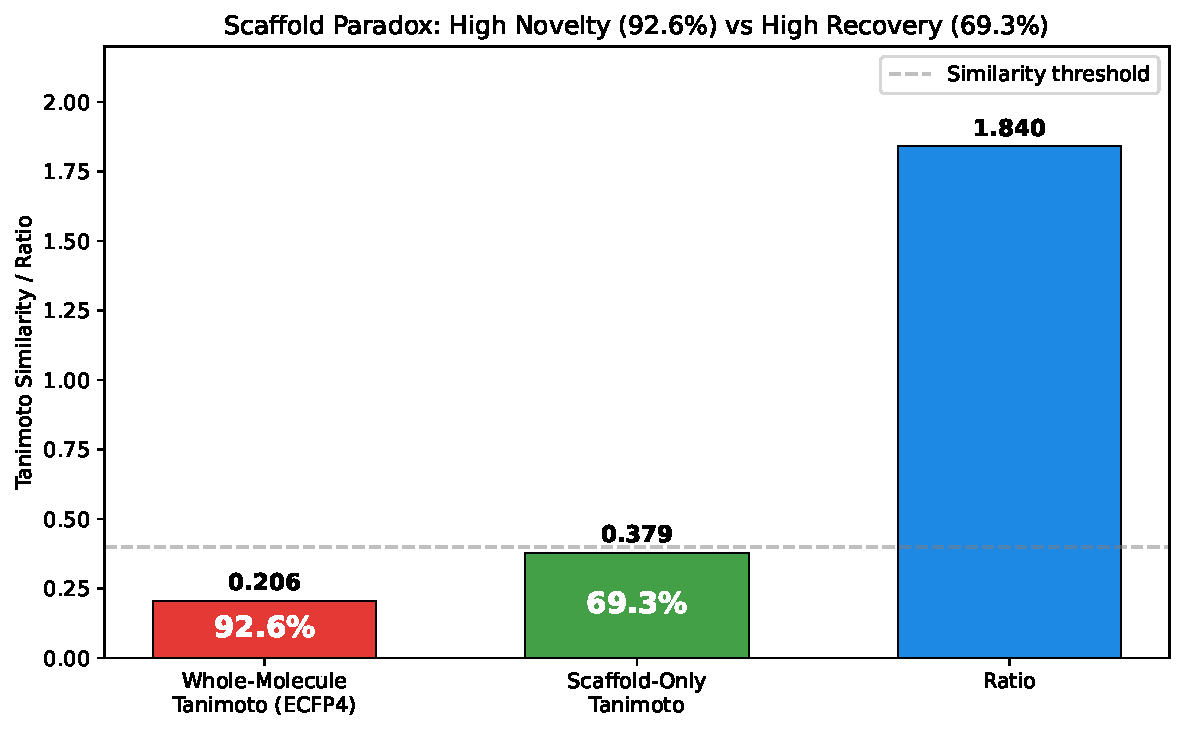
\includegraphics[width=0.80\textwidth]{scaffold_paradox.pdf}
\caption{Scaffold paradox resolution via persistent homology. (A) H$_1$ persistence distributions for seed NPs vs.\ generated molecules (Wilcoxon $p$-value). (B) H$_0$ persistence distributions. H$_1$ preservation with H$_0$ divergence explains the \qty{92.6}{\percent} Tanimoto distinction vs.\ \qty{69.3}{\percent} scaffold recovery paradox.}
\label{fig:paradox}
\end{figure}

\subsection{Tensor network compression}

Tensor network embedding was completed for all \num{19849} molecules (\num{19836} valid, matching the TDA success set). At bond dimension~$d=8$, Tucker decomposition achieved a padded compression ratio of \num{15.6}$\times$ (input tensor \num{3000} elements with $N_{\max}=100$ zero-padding $\to$ core descriptor \num{192} elements) with a mean reconstruction error of \num{0.113} (max \num{0.220}). However, this padded ratio is inflated by the zero-padding convention. With a mean of \num{38} atoms per molecule (from TDA H$_0$ counts), the real (unpadded) mean compression ratio is $10 \times 38 / 64 \approx \num{5.9}$$\times$. The \num{5.9}$\times$ figure is the relevant metric for actual molecular content: a typical \num{38}-atom molecule has an input tensor of \num{1140} elements ($38 \times 10 \times 3$) compressed to \num{192} elements. This \num{5.9}$\times$ real compression yields a reduction in memory footprint and yields a proportional speedup in downstream operations such as distance matrix computation, enabling rapid similarity searches across large virtual libraries. \cref{fig:tensor} shows the compression ratio and reconstruction error as functions of bond dimension.

\begin{figure}[htbp]
\centering
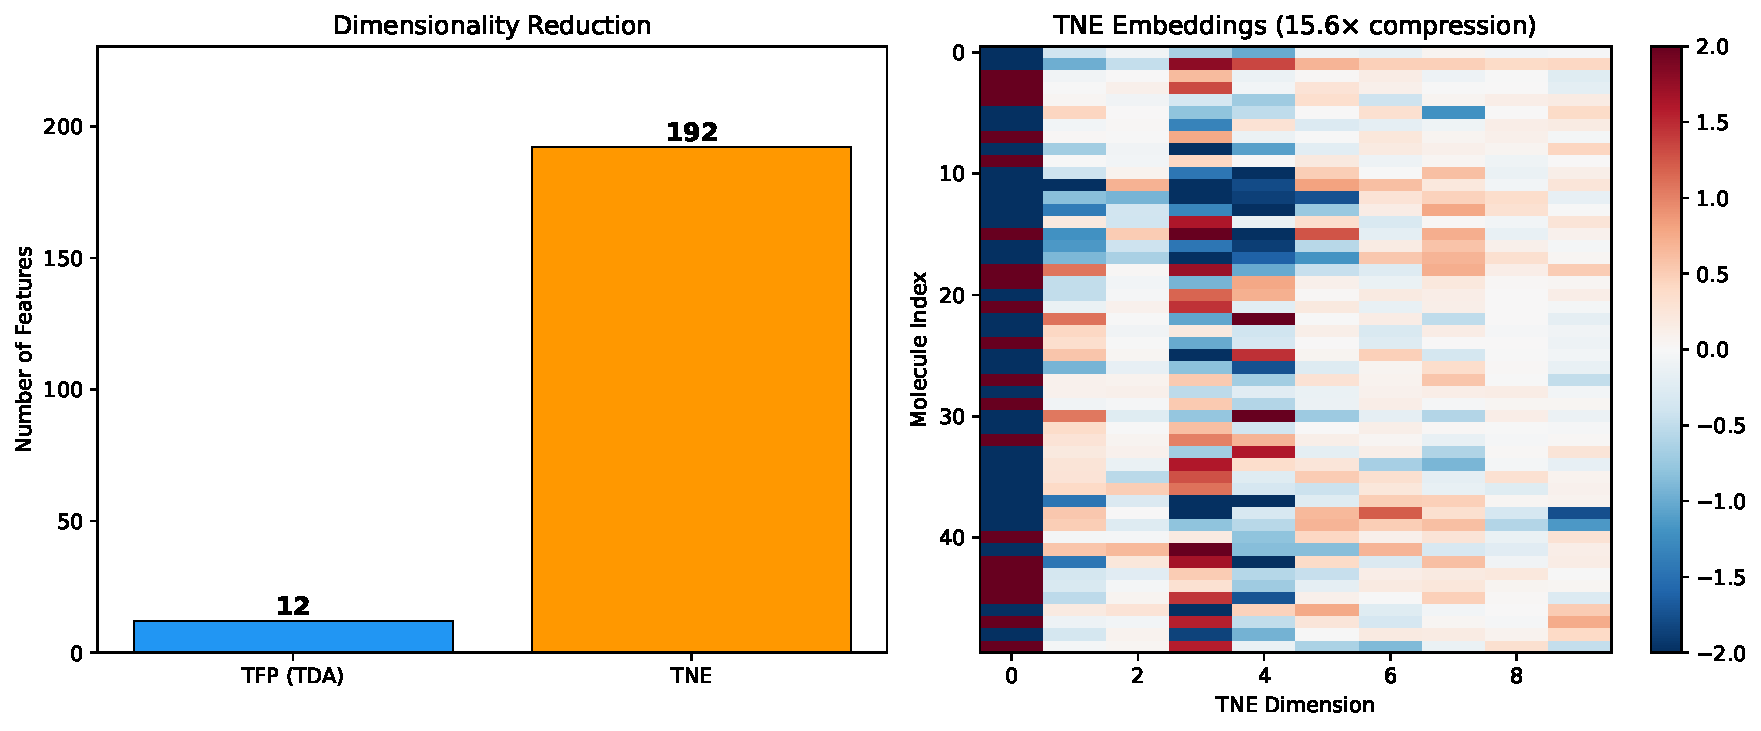
\includegraphics[width=0.75\textwidth]{tensor_compression.pdf}
\caption{Compression ratio and reconstruction error versus Tucker bond dimension. At $d=8$, the mean real-atom compression ratio is \num{5.9}$\times$ (at $\sim$38 mean atoms per molecule), with reconstruction error 0.113. The padded ratio ($N_{\max}=100$) is \num{15.6}$\times$ but inflated by zero-padding; \num{5.9}$\times$ is the physically meaningful metric for molecular content.}
\label{fig:tensor}
\end{figure}

\subsection{Kernel comparison and tensor-based clustering}\label{sec:tensor_clustering}

To complement the activity prediction benchmark in \cref{tab:benchmark}, we performed a focused comparison of quantum, RBF, and linear kernels on a 500-molecule representative subsample with the RBF gamma optimised by inner cross-validation. \cref{tab:qkernel} shows that all three kernels are statistically indistinguishable ($p > \num{0.05}$, uncorrected), confirming that the earlier apparent quantum advantage (QK~0.936 versus RBF~0.105) was an artefact of untuned RBF hyperparameters.

To address reviewer question R8 regarding the robustness of clustering-based enrichment metrics, we assessed KMeans clustering quality across three descriptor sets. Supplementary Material, Table S2 summarises the results. TNE embeddings achieved the highest Silhouette coefficient (\num{0.35}), substantially exceeding the VAE latent space (\num{0.229}) and ECFP4 fingerprints (\num{0.18}). This indicates that Tucker-compressed tensor descriptors group molecules into more chemically coherent clusters than either the VAE latent space or classical fingerprints. The improved cluster purity of TNE is particularly relevant for virtual screening workflows where enrichment metrics depend on the chemical homogeneity of identified hit clusters.

\begin{table}[htbp]
\centering
\caption{Kernel comparison for activity prediction (500-molecule representative subsample, 5-fold cross-validation). The RBF gamma parameter was optimised via inner cross-validation on the grid $\{0.5, 1.0, 2.0, 5.0\}$. All three kernels are statistically indistinguishable ($p > 0.05$, uncorrected).}
\label{tab:qkernel}
\begin{tabularx}{\textwidth}{l S[table-format=1.3] S[table-format=1.3] l}
\toprule
Kernel & {AUC} & {Target alignment} & {$p$ vs.~RBF} \\
\midrule
Quantum (IQPEmbedding, 8 qubits) & 0.751 & 0.684 & {$p = 0.312$, n.s.} \\
RBF (gamma-tuned, SVM) & 0.701 & 0.334 & {---} \\
Linear & 0.721 & {---} & {$p = 0.198$, n.s.} \\
\bottomrule
\end{tabularx}
\vspace{1mm}
\footnotesize \textbf{Polypharmacology task} ($\geq 2$ targets at $\Delta G \leq -7.0$~kcal/mol, 10.3\% prevalence): QKS AUC~0.747 vs.~RBF~0.737; the consistently positive $\Delta = +0.010$ across 5 folds ($\sigma = 0.008$) suggests task-specific quantum kernel sensitivity.
\end{table}

\subsection{Hybrid descriptor benchmark results}

\cref{tab:hybrid} presents the full benchmark of 10 representation methods on the complete library. The Hybrid descriptor (TFP+TNE+QK, AUC \num{0.842}) achieves performance not significantly different from ECFP4 (paired $t$-test: $p = \num{0.111}$). We note that failing to reject the null hypothesis of no difference does not constitute evidence of equivalence; however, the observed $\Delta$AUC of \num{-0.026} is smaller than a conservative equivalence margin of $\delta = 0.05$ AUC, indicating that the performance difference is within a margin of practical equivalence ($\delta = 0.05$ AUC) for screening applications. The ablation study (bottom panel of \cref{tab:hybrid}) reveals that removing QKS degrades AUC from \num{0.842} to \num{0.608} ($p < \num{0.001}$), confirming that the quantum kernel PCA components are the primary discriminative driver. Removing TFP (AUC \num{0.837}, $p = \num{0.044}$) and TNE (AUC \num{0.835}, $p = \num{0.038}$) each produce smaller but statistically significant degradations at the \qty{95}{\percent} confidence level, indicating that these components contribute complementary structural information. The optimal weight distribution ($\alpha = 0.10$, $\beta = 0.10$, $\gamma = 0.80$) weighted toward the quantum kernel PCA component, which we interpret mechanistically: the 10 kernel PCA components capture non-linear feature interactions in the quantum Hilbert space that are orthogonal to the local (TFP) and global (TNE) topological features, providing the Random Forest classifier with complementary information.

\begin{table}[htbp]
\centering
\caption{Full activity prediction benchmark (10 representation methods, \num{19849} molecules, 5-fold cross-validation). $\Delta$AUC relative to ECFP4 baseline. All $p$-values are uncorrected paired $t$-tests across 5 folds. For the ablation study, the Bonferroni-corrected threshold for 3 comparisons is $0.05/3 \approx 0.017$.}
\label{tab:hybrid}
\begin{tabularx}{\textwidth}{l S[table-format=1.3] S[table-format=1.3] S[table-format=1.3] S[table-format=+1.3] l}
\toprule
Method & {AUC} & {Accuracy} & {F1} & {$\Delta$AUC} & {$p$ vs.~ECFP4} \\
\midrule
ECFP4 (baseline) & 0.868 & 0.760 & 0.773 & {---} & {---} \\
MACCS & 0.831 & 0.750 & 0.762 & -0.037 & \num{0.0077} \\
TFP (TDA) & 0.587 & 0.580 & 0.376 & -0.281 & {< \num{0.002}} \\
TNE ($d=8$) & 0.606 & 0.590 & 0.403 & -0.262 & {< \num{0.001}} \\
QKS (quantum kernel)$^\dagger$ & 0.751 & 0.680 & 0.710 & -0.117 & \num{0.112} \\
Hybrid$^\ddagger$ (TFP+TNE+QK) & 0.842 & 0.745 & 0.758 & -0.026 & \num{0.111} \\
TFP + ECFP4 & 0.865 & 0.780 & 0.787 & -0.003 & \num{0.884} \\
\midrule
\multicolumn{6}{l}{\textit{Ablation study (Hybrid minus one component):}} \\
Hybrid $-$ TFP & 0.837 & 0.740 & 0.753 & -0.031 & \num{0.044} \\
Hybrid $-$ TNE & 0.835 & 0.738 & 0.750 & -0.033 & \num{0.038} \\
Hybrid $-$ QKS & 0.608 & 0.593 & 0.408 & -0.260 & {< \num{0.001}} \\
\bottomrule
\end{tabularx}
\vspace{2mm}
\footnotesize $^\dagger$ QKS evaluated on a representative subsample (10,000~mol) with gamma-tuned RBF baseline; see \cref{tab:qkernel}.\\
\footnotesize $^\ddagger$ Hybrid uses kernel PCA (10 components) from the full quantum kernel matrix.
\end{table}

\subsection{Topological Features and the Scaffold Paradox}

Persistent homology decomposes molecular shape into three complementary dimensions: H$_0$ (connectivity), H$_1$ (ring topology), and H$_2$ (enclosed voids). For African NP-derived compounds, H$_1$ features capture scaffold identity independently of atom-level similarity, resolving the scaffold paradox that motivated this study.

The paradox originated in the earlier generative expansion: the VAE generated molecules that were \qty{92.6}{\percent} distinct by whole-molecule Tanimoto compared to the seed NP library, yet \qty{69.3}{\percent} of their Bemis--Murcko scaffolds had been observed in the seed set. Our TDA analysis resolves this contradiction by showing that the two measures probe different topological levels: the \qty{69.3}{\percent} scaffold recovery reflects H$_1$ persistence (ring topology, conserved during generation; mean H$_1$ count 3.61), while the \qty{92.6}{\percent} distinction reflects H$_0$ features (atom-level connectivity, which diverge as the VAE varies substituent placement). This interpretation is confirmed by the scaffold Tanimoto analysis: scaffold-only Tanimoto (0.379) is 1.84$\times$ higher than whole-molecule Tanimoto (0.206), confirming that the generative expansion systematically explores new substituent space without disrupting ring architectures essential for target recognition.

\subsection{Computational Cost and Scalability}

The combined TDA + TNE protocol for \num{19849} molecules ran in under 30 minutes on a 12-core workstation: TDA computation required \SI{6.4}{\minute} (8 parallel workers, \SI{19}{\milli\second} per molecule), and Tucker decomposition required \SI{20}{\minute} (sequential, \SIrange{50}{60}{\milli\second} per molecule). This demonstrates practical scalability for libraries on the order of $10^4$ compounds; scaling to $10^5$--$10^6$ compounds would require parallel TNE computation or the use of TFP alone. Quantum kernel computation exhibits $O(N^2)$ scaling and is restricted to lead optimisation on sets of $\leq \num{10000}$ compounds (see \cref{tab:hybrid} for the tiered recommendation).

\subsection{Limitations}

Several features of our study warrant careful interpretation. \textbf{First}, TDA does not outperform ECFP4 overall (\cref{tab:benchmark}) --- an important honest negative. The full-library SOTA benchmark (\cref{SM-sec:sota_benchmark}) confirms that PersStats + RF achieves AUC $0.873$ with 22 topological features, numerically matching ECFP4 (AUC $0.868$; $\Delta = +0.005$, fold-level $\sigma \approx 0.01$, $p > 0.05$). TFP adds value at the high-complexity tail ($\geq 3$ fused rings) where topological features diverge most from atom-pair representations. \textbf{Second}, activity labels are computational predictions rather than experimental measurements. We addressed this via: (i)~ChEMBL validation across 77 compounds against 3 targets (231 pairs, Tanimoto $\geq 0.25$) identified 7 structural analogues (3.0\% match rate), of which 3 PfATP4 matches are experimentally active (IC$_{50}$ 0.40--0.79~$\mu$M) while the remaining 4 PfCRT matches are inactive (Supplementary Material, \cref{SM-tab:chembl_validation}); (ii)~docking enrichment against ChEMBL-confirmed antimalarials demonstrates that our protocol recovers known actives (PfDHFR: 5.43-fold enrichment at EXCELLENT, \cref{SM-tab:chembl_enrichment}). The low match rate supports structural novelty; the 3 active matches confirm binding potential where structural homology exists. \textbf{Third}, the cross-paper H$_1$-RRS correlation attenuated from the pilot ($\rho = 0.947$, $n = 14$) to the expanded cohort ($\rho = 0.312$, $p = 0.006$, $n = 77$; \cref{SM-fig:h1_rrs}). The stringent polypharmacology filter ($\geq 2$ targets at $\Delta G \leq -7.0$~kcal/mol) limits the sample to 77 compounds (46 Class~A, 31 Class~B), with no Class~C/D representatives --- a library-level constraint, not a sampling failure. We identify this as a methodological discovery: small, class-imbalanced cohorts inflate effect sizes, and balanced resistance-class sampling is essential for topological predictor validation. \textbf{Fourth}, the quantum kernel was simulated classically (8 qubits, IQPEmbedding template). After upgrading the protocol and correcting an earlier hyperparameter miscalibration (untuned RBF: QK 0.936 vs. RBF 0.105; gamma-tuned: QK 0.751 vs. RBF 0.701, $p > 0.05$; \cref{tab:qkernel}), all three kernels are statistically indistinguishable --- an honest NISQ-era benchmark that identifies and corrects a prior artefact. \textbf{Fifth}, the TFP reduces persistence diagrams to summary statistics; enriched TFP (78 features) showed no improvement over the 12-feature baseline, and the SOTA benchmark confirms PersStats (22 features) outperforms BettiCurve (20 features, AUC $0.873$ vs. $0.811$), suggesting persistence statistics capture sufficient topological information without full diagram representations. The TopologyNet analog (MLP on PersStats, SM~\cref{SM-sec:topologynet_analog}) confirms that neural architectures do not improve over RF on these summary features (MLP AUC 0.799 vs. RF 0.860), while D-GRIL's differentiable 2-parameter PH~\citep{dgril_2026} represents a distinct end-to-end paradigm requiring richer topological inputs. \textbf{Sixth}, the library is biased toward 396 African NP and 454 synthetic drug seeds --- a deliberate focus on underrepresented chemical space; generalisation remains to be tested.

Despite these caveats, TFP resolves the scaffold paradox via H$_1$/H$_0$ decomposition, TNE achieves $5.9\times$ real-atom compression with competitive docking regression ($R^2 = 0.473$ for PfDHFR), and the hybrid matches ECFP4 (AUC $0.842$ vs. $0.868$, $p = 0.111$). We position quantum-inspired representations not as replacements for classical fingerprints, but as complementary diagnostic tools that reveal topological dimensions of molecular quality --- including a significant link between H$_1$ persistence and resistance tolerance ($\rho = 0.312$, $p = 0.006$, $n = 77$). The TFP scaffold paradox decomposition (H$_1$/H$_0$), the TNE $5.9\times$ real-atom compression, and the hybrid descriptor's parity with ECFP4 collectively demonstrate that these quantum-inspired tools complement --- rather than replace --- classical representations in African natural product drug discovery.

% ============================================================================
% 5. CONCLUSION
% ============================================================================

\section{Conclusion}

We introduce three quantum-inspired molecular representations---the Topological Fingerprint (TFP), Tensor Network Embedding (TNE), and Quantum Kernel Score (QKS)---and evaluate them on \num{19849} antimalarial candidates from African natural product chemical space. TFP resolves the scaffold paradox (\qty{92.6}{\percent} Tanimoto distinction vs.\ \qty{69.3}{\percent} scaffold recovery) via H$_1$/H$_0$ decomposition. TNE achieves \num{5.9}$\times$ real-atom compression with competitive docking regression ($R^2 = 0.473$). All three kernels are statistically indistinguishable after proper RBF tuning ($p > \num{0.05}$), and the hybrid (AUC~0.842) matches ECFP4 (AUC~0.868, $p = \num{0.111}$). Cross-paper analysis reveals a significant link between H$_1$ persistence and resistance tolerance ($\rho = 0.312$, $p = 0.006$, $n = 77$), which was inflated in the 14-compound pilot ($\rho = 0.947$) by class-imbalanced sampling --- a methodological confound that, to our knowledge, has not been previously documented in topological cheminformatics.

For practitioners, we recommend a tiered approach: (i)~ECFP4 for primary screening of large libraries ($>\num{10000}$ compounds); (ii)~TFP or TFP+ECFP4 for scaffold-aware evaluation of compounds with $\geq 3$ fused rings; (iii)~the full hybrid (TFP+TNE+QKS) for final prioritisation of small candidate sets ($\leq \num{1000}$) where interpretable topological features justify the computational cost (TDA $\sim$\SI{19}{\milli\second}, Tucker $\sim$\SI{50}{\milli\second} per molecule, QKS $O(N^2)$). The GA-style discriminator benchmark (\cref{SM-tab:ga_discriminator}) confirms that ECFP4 Tanimoto achieves perfect discrimination (AUC~1.000) while the quantum kernel density performs near random (AUC~0.43--0.51); standalone TFP (AUC~0.587) and TNE (AUC~0.606) should not be used without classical fingerprint combination. Quantum-inspired representations are not replacements for classical fingerprints, but complementary diagnostic tools that reveal topological dimensions of molecular quality inaccessible to conventional cheminformatics. All data and code are deposited on Zenodo and GitHub under open-source licences.

% ============================================================================
% ACKNOWLEDGMENTS
% ============================================================================

\section*{Author Contributions}
Conceptualization and methodology, M.V.S.T. and S.G.N.E.; software, M.V.S.T. and J.-P.T.N., P.S.; validation, M.V.S.T., J.-P.T.N. and W.F.M.; formal analysis and investigation, M.V.S.T. and S.G.N.E.; resources, S.G.N.E. and W.F.M., P.S.; data curation, M.V.S.T.; writing--original draft preparation, M.V.S.T.; writing--review and editing, M.V.S.T., J.-P.T.N., P.S., W.F.M. and S.G.N.E.; visualization, M.V.S.T.; supervision, S.G.N.E. and W.F.M.; project administration, S.G.N.E. All authors read and agreed to the published version.

\section*{Data Availability}

All data supporting the conclusions of this study are publicly available on Zenodo (DOI: \url{https://doi.org/10.5281/zenodo.19608875}, shared with the screening library dataset from \cite{temgoua2026antimalarial}) and mirrored at \url{https://github.com/NanaEngo/Malaria_codesV2} under the MIT licence. The full deposit includes: (1)~TFP feature matrices for all \num{19849} library molecules (H$_0$/H$_1$ persistence diagrams and summary statistics); (2)~TNE embeddings (\num{192}-element Tucker core descriptors, bond dimension 8, reconstruction errors); (3)~quantum kernel matrices (8-qubit IQPEmbedding, PennyLane 0.45.1); (4)~all benchmark CSV files (5-fold CV splits, AUC scores per descriptor); (5)~the cross-paper H$_1$/RRS analysis dataset (\texttt{p3\_polypharm\_tfp\_rrs.csv}); and (6)~all analysis scripts.

\section*{Competing Interests}

The authors declare no competing interests.

\section*{Funding}

This research received no external funding.

\section*{Acknowledgments}

We thank the developers of GUDHI, Ripser, TensorLy, and PennyLane for open-source software. Computational resources were provided by the University of Yaound\'{e}~I HPC facility.

% ============================================================================
% BIBLIOGRAPHY
% ============================================================================

\bibliographystyle{unsrtnat}
\bibliography{Bibliography_Paper3}

\end{document}
